\scanpage{31}
% paper watermark, sideways, first fragment clipped at the upper edge
{\centering \textsc{\unsure{Extr}\unsure{a}}\\
\textit{\unsure{Ma}\unsure{in|i|nn}}\par}
\figure{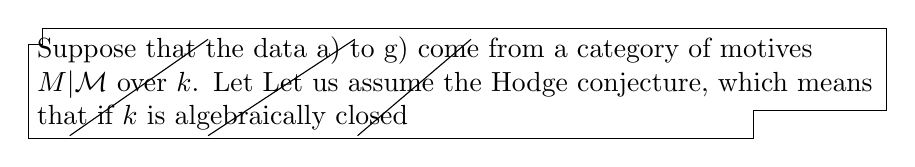
\begin{tikzpicture}[x=1cm,y=1cm]
\node[inner sep=3pt,text width=.88\linewidth,align=left] (oldblock) {\deleted{Suppose that the data a) to g) come from a category of motives $\unsure{M|\mathcal M}$ over $k$. \deleted{\unsure{Let}} Let us assume the Hodge conjecture, which means that if $k$ is algebraically closed}};
\draw ([xshift=5pt]oldblock.north west) -- (oldblock.north east) -- ([yshift=10pt]oldblock.south east) -- ([xshift=-48pt,yshift=10pt]oldblock.south east) -- ([xshift=-48pt]oldblock.south east) -- (oldblock.south west) -- ([yshift=-6pt]oldblock.north west) -- ([xshift=5pt,yshift=-6pt]oldblock.north west) -- cycle;
\draw ([xshift=15pt,yshift=1pt]oldblock.south west) -- ([xshift=65pt,yshift=-4pt]oldblock.north west);
\draw ([xshift=65pt,yshift=1pt]oldblock.south west) -- ([xshift=118pt,yshift=-4pt]oldblock.north west);
\draw ([xshift=119pt,yshift=1pt]oldblock.south west) -- ([xshift=160pt,yshift=-4pt]oldblock.north west);
\end{tikzpicture}}

Let $V_{\mathbb Q},\ V_{\mathbb C}=\sum_{pq}V^{pq}$ be a Hodge structure, and let $G$ be its Mumford-Tate group, thus $G_{\mathbb C}\subset\underline{\mathrm{Aut}}_{\mathbb C}(V)$. Let $V_k\subsetV_{\mathbb C}$ be a restriction of scalars from $\mathbb C$ to $k\subset\mathbb C$, \deleted{\unsure{a}} \uline{compatible} with the natural filtration of $V_{\mathbb C}$. Suppose that $(V_{\mathbb Q},\,V_{\mathbb C}=\sum V^{pq},\,V_k\subset V_{\mathbb C})$ comes from a motive over \uuline{$k$}. \inserted{\deleted{Assuming}} \deleted{and let us assume the \unsure{Hodge|Hodge} conjecture} \deleted{Then}

The motivic Galois group of the latter, relative to $T_{\mathrm{DR}}$, is \unsure{a|a} \deleted{form} \inserted{group} $G'$ \unsure{defined} over $k$, \deleted{of $G_{\mathbb C}$,} and by virtue of \uline{Hodge conjecture} one must have $G'_{\mathbb C}\unsure{=|\subset}G^\circ_{\mathbb C}$. \deleted{(\unsure{according to} \illegible{2})} In other words, $G^\circ_{\mathbb C}$ must be ``definable over $k$ via $V_k\subset V_{\mathbb C}$'' ; this is a very ; highly nontrivial condition ! When $k$ is algebraically closed, one will need \deleted{\unsure{in}} $G'_{\mathbb C}=G_{\mathbb C}$, which can be expressed by saying that $\unsure{\forall|H}$ \deleted{invariant} element of a ${\bigotimes}_{\mathbb Q}^{\unsure{n|m}}(V'\otimes_{\mathbb Q}V)$ invariant under $G$ (i.e. of bidegree $0$) is necessarily in $\bigotimes_{\unsure{k'|\bar k}}^{\unsure{n|m}}(V'_{\unsure{k'|\bar k}}\otimes_{\bar k}V_{\unsure{k'|K'}})$\unsure{!} ; if $k$ general, one must \deleted{replace $k$ by an extension} \inserted{therefore $\exists$ finite extension $k'$ of $k$,} having the preceding virtue. These are again very restrictive conditions on the structure envisaged. They are certainly not sufficient (take $k=\mathbb Q$, $V_k=V_{\mathbb Q}$, this is in general not possible
\figure{\begin{tikzpicture}[x=1pt,y=1pt]
\draw[dash pattern=on 8pt off 4pt] (0,0) -- (49,0);
\draw (55,6) -- (60,6) -- (61,0) -- (55,0);
\end{tikzpicture}}
% paper watermark, sideways, second fragment clipped at the lower edge
{\centering \textsc{\unsure{Strong}}\\
\textit{\unsure{uy|ny|y} \unsure{1808}}\par}
% archive sheet number: 30
